In the above content, the mathematical properties of OFDM is elegant but the real life application could be complex. For example, how to align the received signal with the transmitted signal? How to detect the number of multipath in the channel? How to detect the frequency offset and align subcarriers? The above questions are referring synchronization and channel estimation. In this section, we will discuss the related techniques.

\subsection{Synchronization}
In designing the optimal receiver, a matched filter containing possible transmitted waveforms is used to classify the received signal. However, the OFDM baseband signal $x(t)$ is a superposition of multiple subcarriers' data symbols by the Inverse Fourier transform. And the matched filter is actually applied on the Fourier transform of the received signal $\mtx{Y}$. To guarantee the optimal performance, the receiver should be able to align the FFT operator with the observed sample stream. This process is time synchronization.

The time synchronization of the OFDM system can be achieved by a correlation-based approach. Due to the usage of cyclic prefix, signal contains a part of repeated pattern of itself. The receiver can calculate the sliding autocorrelation of the observed symbol stream using a lag commensurate with the length of the cyclic prefix. The magnitude of the result will reach a peak (close to 1) at the instant the corresponds to the end of the cyclic prefix, which is also the start of the desired signal. The limitations of the correlation based synchronization is that it does not optimize SNR. There are other methods to achieve time synchronization, such as the MLE/MAP/MMSE, \etc in corporate with the cyclic prefix for balanced performance.

% The OFDM system also needs frequency synchronization, which helps align the frequency offset between the transmitter and the receiver. Since the subcarriers are transmitted in parallel, frequency synchronization can help the demodulated signal maintain the same 

The OFDM system also needs frequency synchronization because the subcarriers are frequency relevant. A common approach is using Phase-locked loop (PLL)~\cite{ContributorstoWikimediaprojects2024Mar}. The intuition behind the PLL is that any consecutive two samples are supposed to have the same phase shift in an LTI system. So we can generate a compensation phase shift to align the incoming signals. The compensation phase shift will be used to generate a reference signal to be compared with the next input signal and then update the compensation phase shift by averaging all the previous phase shifts. Once the compensation phase shift stop changing, the optimal result of the PLL is achieved.

The OFDM system is less sensitive to the time synchronization so the mentioned technique is usually adequate. But the frequency synchronization is more critical and challenge. To achieve high resolution frequency synchronization result, the knowledge of the channel is preferred. This process is channel estimation, and it can be done at the receiver with the help of pilot symbols.

\subsection{Pilot Symbols}
The Pilot Symbols are data symbols, which are known by transmitter and receiver, inserted into the transmitted signal. The receiver can use the known data symbols to estimate the channel and then compensate the channel effect on the received signal or perform synchronization.

There are many ways to insert the pilot symbol. It can be interpolated purely in between time slots, in between frequency spacing, or in between both.
\begin{enumerate*}[(i)]
    \item If the pilot symbol is added on the $k$-th subcarrier, while the received signal detect the pilot symbol on the $k'$-th subcarrier, the receiver can estimate the frequency offset by the difference of $k$ and $k'$;
    \item If the pilot symbol is added on the $l$-th time slot, while the received signal detect the pilot symbol on the $l'$-th time slot, the receiver can estimate the time offset by the difference of $l$ and $l'$;
    \item If the pilot symbol has magnitude $A$, while the received signal detect the pilot symbol with magnitude $A'$, the receiver can estimate the channel gain by the ratio of $A$ and $A'$.
\end{enumerate*}

The pilot symbol method is an effective and flexible technique. The occupancy of bandwidth does reduce the spectral efficiency, but the performance gain is significant. The pilot symbol method is widely used in the OFDM system. The channel estimation not only helps the synchronization but also improves the performance of other signal processing techniques, such as equalization, beamforming, and precoding. The~\cref{fig:pilot} shows the channel estimation aided by pilot symbols.

\begin{figure}[!htbp]
    \centering
    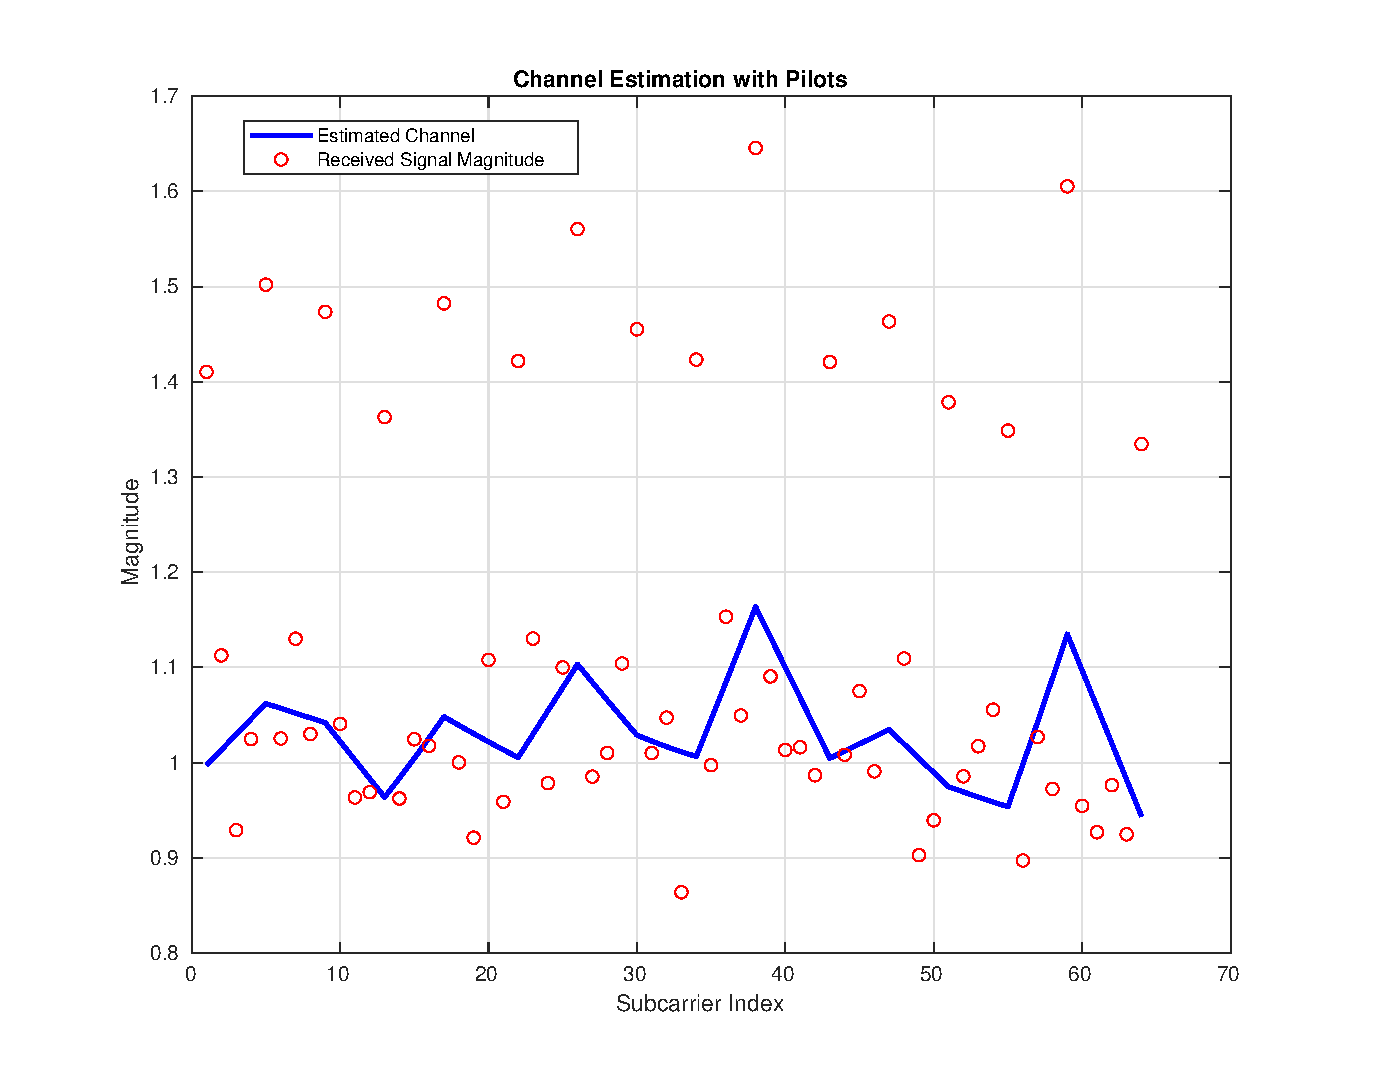
\includegraphics[width=\linewidth]{Pilot.eps}
    \caption{BPSK, $64$ subcarriers, $16$ CP, $1000$ OFDM symbols, pilot value $1+1j$}
    \label{fig:pilot}
\end{figure}